\frame{
  \begin{block}{Overall architecture}
    
    \begin{itemize}
    \item \alert{ProM} an existing process analysis framework
    \item \alert{OpenSPCoop} the most adopted  open source SPCoop implementation
    \end{itemize}

  \end{block}
  \begin{center}
    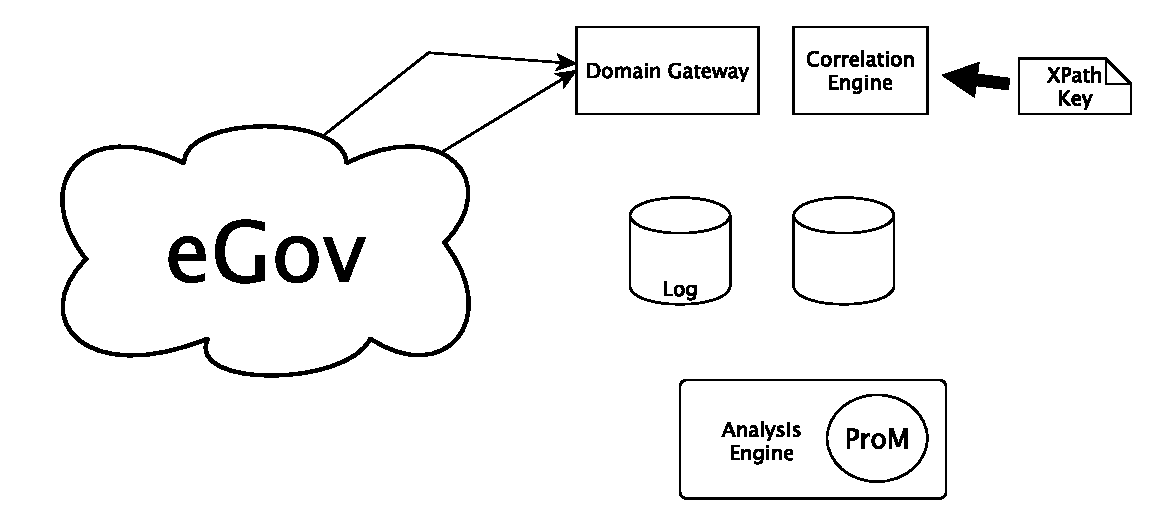
\includegraphics[scale=0.30]{./fig/Platform01}
  \end{center}

}

\frame{
  \begin{block}{Overall architecture}
    
    \begin{itemize}
    \item \alert{ProM} an existing process analysis framework
    \item \alert{OpenSPCoop} the most adopted  open source SPCoop implementation
    \end{itemize}

  \end{block}
  
  \begin{center}
    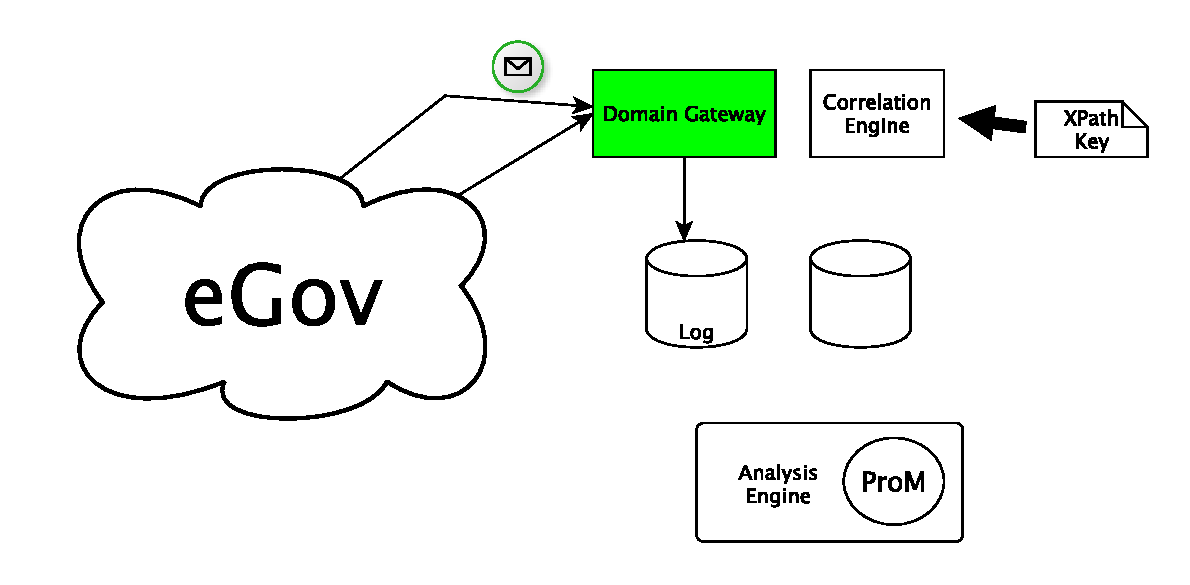
\includegraphics[scale=0.30]{./fig/Platform02}
  \end{center}

  \begin{itemize}
    \item eGov envelopes intercepted by Domain Gateway
    \item Domain Gateway stores message key information into the Log
      database
    %\item Domain Gateway performance are not affected by the analysis
    % \item <2-> Correlation engine groups SOAP request/response
    %   \begin{itemize}
    %     \item exploiting correlation sets (\alert{XPath})
    %     \item annotates process instances into log requests
    %     \item is externally triggered (e.g. cron/trigger)
    %   \end{itemize}
    % \item <3-> Analysis engine evaluates process metrics
    %   \begin{itemize}
    %     \item process definition stored in an external database (\alert{BPMN})
    %     \item process metrics stored into the log database
    %     \item is externally triggered (e.g. cron/trigger)
    %     \item fuffa su ProM
    %   \end{itemize}
  \end{itemize}
}

\frame{
  \begin{block}{Overall architecture}
    
    \begin{itemize}
    \item \alert{ProM} an existing process analysis framework
    \item \alert{OpenSPCoop} the most adopted  open source SPCoop implementation
    \end{itemize}

  \end{block}
  
  \begin{center}
    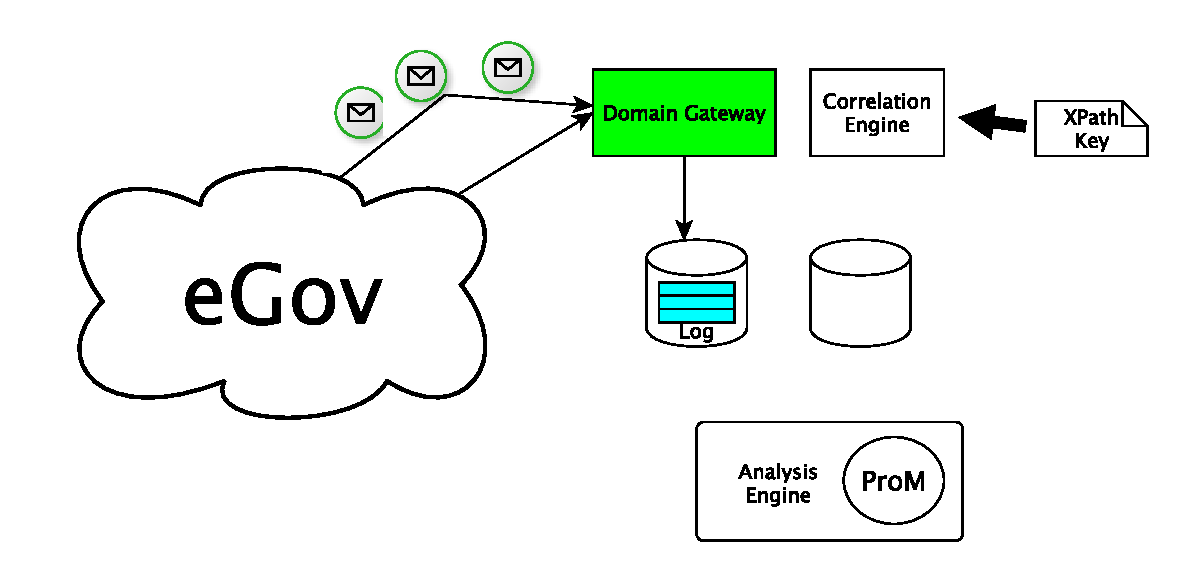
\includegraphics[scale=0.30]{./fig/Platform03}
  \end{center}

  \begin{itemize}
    \item eGov envelopes intercepted by Domain Gateway
    \item Domain Gateway retrieves messages parts storing into the Log
      database
    %\item Domain Gateway performance are not affected by the analysis
    % \item <2-> Correlation engine groups SOAP request/response
    %   \begin{itemize}
    %     \item exploiting correlation sets (\alert{XPath})
    %     \item annotates process instances into log requests
    %     \item is externally triggered (e.g. cron/trigger)
    %   \end{itemize}
    % \item <3-> Analysis engine evaluates process metrics
    %   \begin{itemize}
    %     \item process definition stored in an external database (\alert{BPMN})
    %     \item process metrics stored into the log database
    %     \item is externally triggered (e.g. cron/trigger)
    %     \item fuffa su ProM
    %   \end{itemize}
  \end{itemize}
}

\frame{
  \begin{block}{Overall architecture}
    
    \begin{itemize}
    \item \alert{ProM} an existing process analysis framework
    \item \alert{OpenSPCoop} the most adopted  open source SPCoop implementation
    \end{itemize}

  \end{block}
  
  \begin{center}
    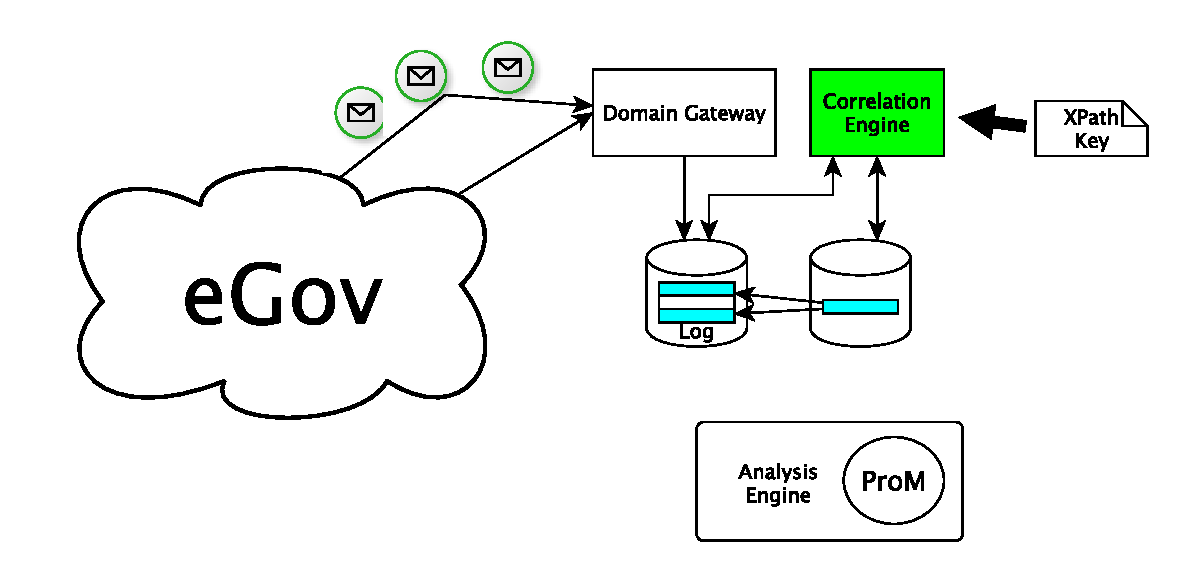
\includegraphics[scale=0.30]{./fig/Platform04}
  \end{center}

  \begin{itemize}
    \item Correlation engine groups SOAP request/response
       exploiting correlation sets (\alert{XPath})
     \item Service externally invoked (e.g. cron/trigger)
    % \item <3-> Analysis engine evaluates process metrics
    %   \begin{itemize}
    %     \item process definition stored in an external database (\alert{BPMN})
    %     \item process metrics stored into the log database
    %     \item is externally triggered (e.g. cron/trigger)
    %     \item fuffa su ProM
    %   \end{itemize}
  \end{itemize}
}

\frame{
  \begin{block}{Overall architecture}
    
    \begin{itemize}
    \item \alert{ProM} an existing process analysis framework
    \item \alert{OpenSPCoop} the most adopted  open source SPCoop implementation
    \end{itemize}

  \end{block}
  
  \begin{center}
    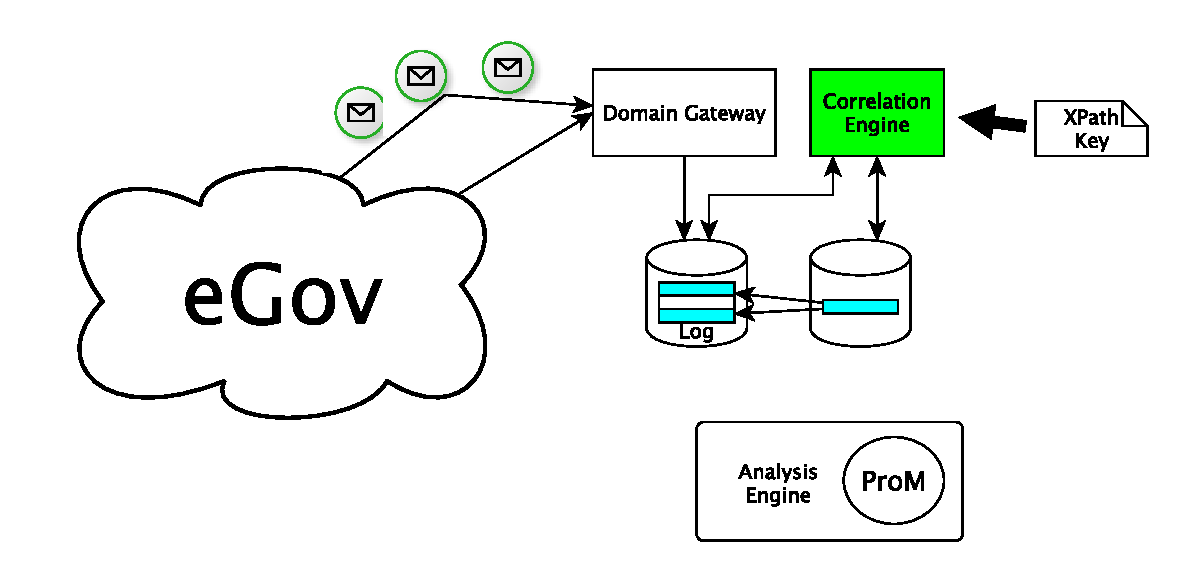
\includegraphics[scale=0.30]{./fig/Platform04}
  \end{center}

  \begin{itemize}
    \item Analysis engine evaluates process metrics
    \item Service externally invoked (e.g. cron/trigger)
    \item implements a context to integrate ProM into JBoss AS
  \end{itemize}
}

%%% Local Variables: 
%%% mode: latex
%%% TeX-master: "main"
%%% End: 
